\documentclass[12pt]{article}
\usepackage[paper=letterpaper,margin=2cm]{geometry}

%\usepackage{coffeestains} %lmao

\usepackage{amsmath}
\usepackage{amsthm} %needed for the proofs 
\usepackage{amssymb}
\usepackage{titling}
\usepackage{thmtools}
\usepackage{mathptmx} %font
\usepackage{verbatim} % for comments
\usepackage{mdframed}
\usepackage[linesnumbered,ruled,vlined]{algorithm2e}
\usepackage{lipsum}
\usepackage{listings}

\lstset{
  basicstyle=\ttfamily,
  columns=fullflexible,
  frame=single,
  breaklines=true
}

% --- NAMES --- %
\newcommand{\nameone}{Alexandre St-Aubin}
\newcommand{\nametwo}{ and Jonathan Campana}
%images
\usepackage{graphicx}
\graphicspath{ {./graphics/} }
% to include an image, do: 
%    \begin{center}
%    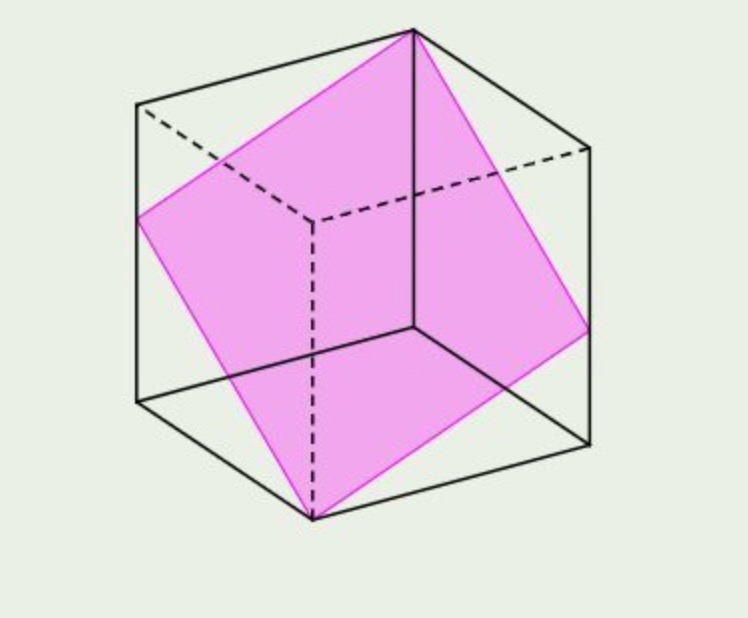
\includegraphics[scale=0.20]{graph.jpg}
%    \end{center}
% OR: 
%\begin{figure}
%    \centering
%    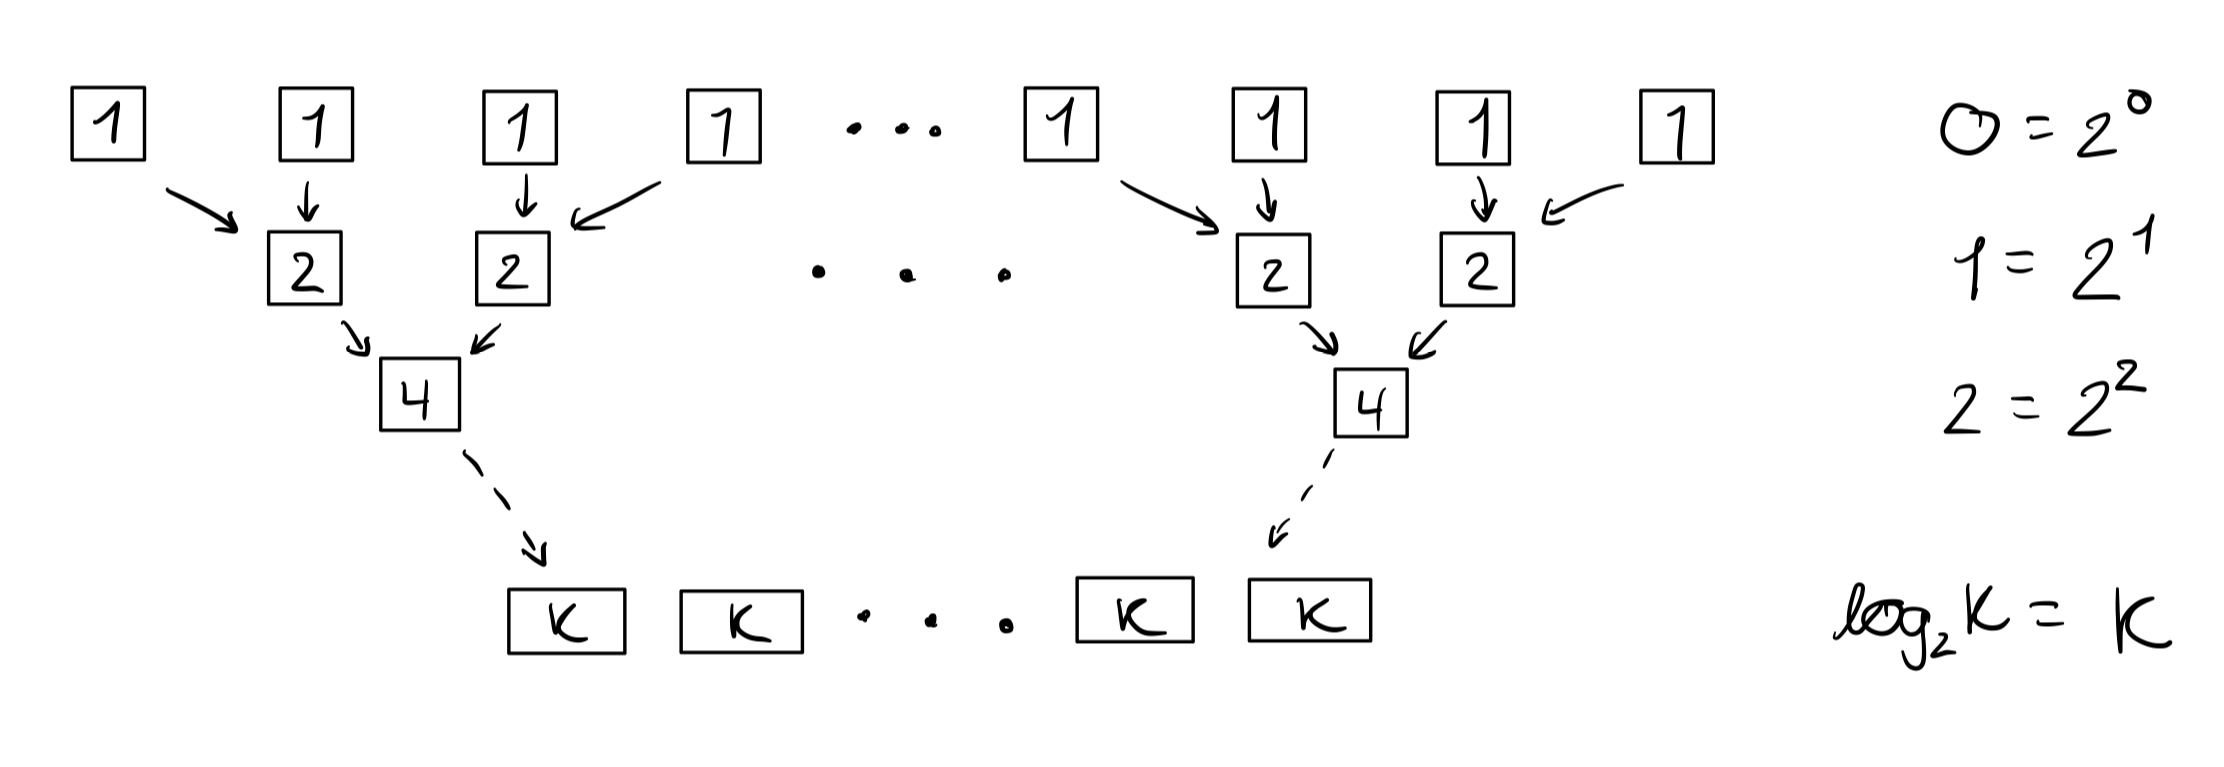
\includegraphics[scale=0.20]{IMG_1052.jpg}
%    \caption{Your caption text here.}
%\end{figure}


%For plots
\usepackage{pgfplots}
\pgfplotsset{compat = newest}

% --- Custom Math Commands --- %
\newtheorem{theorem}{Theorem}
\declaretheoremstyle{lemma}
\declaretheorem[style=lemma, name=Lemma]{lemma}

\theoremstyle{definition}
\newtheorem{definition}{Definition}

\declaretheoremstyle{example}
\declaretheorem[style=example, name=Example]{example}

\theoremstyle{remark}
\newtheorem*{remark}{Remark}

\declaretheoremstyle{proposition}
\declaretheorem[style=proposition, name=Proposition]{proposition}

\declaretheorem[name=Note]{note}
\declaretheoremstyle{note}

\newenvironment{ftheo}
  {\begin{mdframed}\begin{theorem}}
  {\end{theorem}\end{mdframed}}


  % --- Special commands --- %
\newcommand\sol{%
  \\ 
  \\
  \textit{Solution:}\\%
}
% Statistics
\newcommand{\indep}{\perp \!\!\! \perp}
\DeclareMathOperator{\var}{Var}
\DeclareMathOperator{\cov}{Cov}

%Convex optimisation operators
\DeclareMathOperator{\epi}{epi}
\DeclareMathOperator{\lev}{lev}
\DeclareMathOperator{\dom}{dom}
\DeclareMathOperator{\aff}{aff}
\DeclareMathOperator{\ri}{ri}
\DeclareMathOperator{\argmin}{argmin}
\DeclareMathOperator{\conv}{conv}
\DeclareMathOperator{\cl}{cl}


% --- Header --- %
%\renewcommand{\headrulewidth}{.4mm} % header line width

\usepackage[T1]{fontenc} %header
\usepackage[utf8]{inputenc}%header
\usepackage{geometry} %header
\usepackage{fancyhdr}%header
\usepackage{blindtext}
\usepackage{lastpage}

\pagestyle{fancy}
\fancyhf{}
\fancyhfoffset[L]{1cm} % left extra length
\fancyhfoffset[R]{1cm} % right extra length
\rhead{\today}
\lhead{\it \nameone \nametwo}
\fancyfoot[R]{Page \thepage \hspace{1pt} of \pageref{LastPage}}

% --- Title Page --- % 
\setlength{\droptitle}{-6em}

\title{\textsc{Assignment 4 -- COMP 252}}  
\author{\it \nameone \nametwo}
\date{\today}

\begin{document}
\maketitle 
\thispagestyle{empty} %clear first page numbering
%\coffeestainA{0.9}{0.85}{-25}{5cm}{1.3cm}
\begin{enumerate}
  \item \textsc{Browsing the small elements in a red-black tree}. Given is an ordinary red-black tree with a pointer to the smallest element (in addition to a pointer to the root). Cells have five components: left, right, and parent pointers, color of the node, and value of the key.
\begin{enumerate}
  \item We are asked to search for an element u in the tree with key key [u] = x. Show that this can
be done in time $O(1 + \log(k))$ if $x$ is the $k$-th smallest key value stored in the tree (but we only know $x$, not $k$).
\sol
Given a red black tree, we have a balanced binary tree. This means that we can find any element in the RB tree in $\log_2(n)$ time. This also means that we have at most $\lceil \log_2(n)\rceil$ levels to our tree. 

Therefore, starting at the smallest node, we work our way up the RB tree by checking if the key of the node we are at is smaller than the node we are looking for (x). We keep doing this until we find a node that has a key that is bigger than the key we are looking for, or we reach a node that does not have a parent nodes (the root). This is the lowest common ancestor with the $k^{th}$ smallest node. 


Denote the lowest common ancestor as the node that is ancestor to the $k^{th}$ smallest node and the smallest node (our starting point). Given that our nodes are ordered in a red black tree, the possible lowest common ancestors (we will refer to them as LCAs from now on) would be found as the most left nodes of the tree at each level. Denote the possible LCAs
\begin{align*}
    LCA = \{v_1, v_2, \ldots, v_{n}\}
\end{align*}
By the red black tree, we have $\log(n)$ possible LCAs since the tree has n nodes. We, however, will not always reach the root, which is why our complexity is dependent on the $k^{th}$ smallest element rather than $n$. 

By our algorithm, we move to the parent as long as the element we are looking for is bigger than the parent of the node we are currently at. Once we reach the point where the $k^{th}$ smallest element is smaller than the parent node, or the parent node does not exist (the root), we conclude that the element we are searching for must be in the right subtree of the node we are at. 

The $k^{th}$ smallest element in the binary tree can be any element in the right subtree including the current node for the sake of simplicity. Suppose that our LCA is $v_i$. Since the node that contains $k$ is in the right subtree, and the subtree with $v_i$ as the LCA would have at most $2k$ elements inside. 

This is easy to see since the lower bound for the number of leaves in the $v_i$ would be $2k$ (in big Oh) if $key[v_i] = k$, then the left subtree would have $k-1$ elements since that is the number of elements smaller than the node we are looking for, and the right subtree would have at most $k-1$ nodes as well. Suppose that $k$ was farther inside the right subtree, $k$ would be bigger than in the previous case, we could take without loss of generality that the $v_i$ subtree has $2k$ nodes (even though it would have less, since the left subtree wouldn't have k nodes in it) which would give us the same $O(\log(k))$, since the number of levels in this red black $v_i$ subtree is $\lceil \log_2 k \rceil$. 


The second while loop essentially binary searches the right subtree of our LCA $v_i$, which has at most $k$ many nodes in it. Since it takes $O(\log k )$ to binary search a red black tree, this while loop also has $O(\log k)$.

Thus, employing the triangle inequality with this distance metric, we have that 
\begin{align*}
    &d(\text{min pt, } k^{th}) \le d(\text{min pt, greatest common ancestor}) + d(\text{greatest common ancestor, } k^{th}) + 1\\
    &\implies d(\text{min pt, } k^{th}) \le O(\log k + 1) + O(\log k) = O(\log k + 1)\\    
\end{align*}

The constant in our big Oh notation stems from the possibility that $k=1$, where $\log k = 0$, but there is still a comparison, so we add the 1. 

  \item[\it (ii)] Give the algorithm for part (i).

\begin{algorithm} 
    \caption{Find\_kth\_smallest red-black tree.}
    \SetKwProg{Fn}{Function }{\string:}{}
    \SetKwRepeat{Do}{do}{while} %do-while loop macro
    \SetKwInput{KwOut}{Output}
    \SetKwInput{KwIn}{Input}
    \SetKwFunction{rad}{Radius}
    \SetKwFunction{cen}{centre\_dist}
    \SetKwData{dec}{possible\_adjacent\_stack}
    \SetKwData{a}{a}
    \SetKwData{b}{b}
    \SetKwData{np}{node\_pointer}    
    \SetKwData{ltok}{left\_to\_circle}   
    \SetKwData{maxd}{max\_d}   
    \SetKwData{null}{NULL}  
    \SetKwData{wid}{Width}   
    \SetKwFunction{mn}{MAKENULL}
    \SetKwFunction{top}{PEEK}
    \SetKwFunction{pop}{POP}
    \SetKwFunction{push}{PUSH}

    \KwIn{Pointers to the smallest element and root of a red black tree, and value of $x$. }
    \KwOut{Finds node of value $x$ in the tree.}
    \BlankLine
    \While{$(x \geq \text{key}[\np])$}{
        \If{$\text{key}[\np] = x$}{
             \Return $\np$;
        }
        \eIf{$(\text{key}[\text{parent}[\np]] \neq \null)$}{
            $\np \gets \text{parent}[\np]$;
        }{
        \textbf{break};
        }
   }    
    $\np \gets \text{right}[\text{left}[\np]]$ \tcp{\color{blue}The parent was bigger than $x$, thus we go back in the subtree and set our pointer to the right child}
    
    \While{$(x \neq \text{key}[\np]) \land (\text{key}[\np] \neq \null)$}{
        \eIf{$x > \text{key}[\np]$}{
            $\np \gets \text{right}[\np];$
        }{
        $\np \gets \text{left}[\np];$
        }
    }
    
    \eIf{$x = \text{key}[\np]$}{
      \Return $\np$;
    }{
       \Return \null;
    }
    
\end{algorithm}
\end{enumerate}
  \newpage 
  \item \textsc{Greedy algorithm}. On a flat table, we have placed n disks of radii $r_1, ..., r_n$, numbered from left to right. We push them together without creating overlap, as in the figure below. Give an $O(n)$ time algorithm to compute the size of the smallest axis-aligned rectangle that can hold the disks.
  \sol 
  See the algorithm on the next page. We show that its complexity is $O(n)$. To begin, the outermost loop at line 8 iterates a total of $n$ times. The maximum number of elements pushed onto the stack is also $n$ (since at most one is pushed at each iteration), hence an equal number is removed, maintaining the overall $O(n)$ complexity. Finally, as we traverse through each circle once more at the end of the algorithm, the complexity remains $O(n)$.
\begin{figure}[htb!]
     \centering
     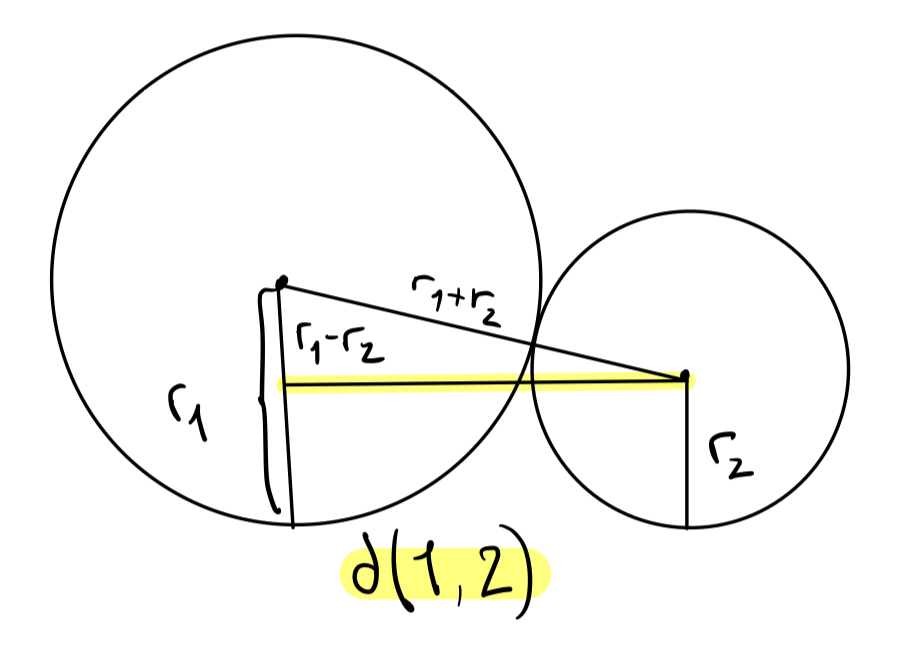
\includegraphics[scale=0.20]{A4-252.jpg}
     \caption{The distance calculated by \texttt{centre\_dist()} in \textbf{Algorithm 2}.} 
\end{figure}

  \begin{algorithm}
    \caption{Greedy circle packing}
    \SetKwProg{Fn}{Function }{\string:}{}
    \SetKwRepeat{Do}{do}{while} %do-while loop macro
    \SetKwInput{KwOut}{Output}
    \SetKwInput{KwIn}{Input}
    \SetKwFunction{rad}{Radius}
    \SetKwFunction{cen}{centre\_dist}
    \SetKwData{dec}{possible\_adjacent\_stack}
    \SetKwData{a}{a}
    \SetKwData{b}{b}
    \SetKwData{arr}{array}    
    \SetKwData{ltok}{left\_to\_circle}   
    \SetKwData{maxd}{max\_d}   
    \SetKwData{len}{length}  
    \SetKwData{wid}{Width}   
    \SetKwFunction{mn}{MAKENULL}
    \SetKwFunction{top}{PEEK}
    \SetKwFunction{pop}{POP}
    \SetKwFunction{push}{PUSH}

    \KwIn{An ordered list $\Omega := \{1,2,3,...,n\}$ of $n$ circles. }
    \KwOut{The minimum width of a rectangle that can hold the disks.}
    \BlankLine

    \tcp{\color{blue}radius of the circle a}
    \Fn{\rad{circle \a}}{
        \Return radius of \a;
    }
    \BlankLine

    \tcp{\color{blue}distance between the centres of a and b if they are pushed together.}
    \Fn{\cen{circle \a, circle \b}}{
      \Return $ \sqrt{(\rad(a)+\rad(b))^2 -(\rad(a)-\rad(b))^2};$
    }
    \BlankLine 
    \tcp{\color{blue} Stack of possible adjacent circles.}
    $\mn (\dec); $\\
    \BlankLine 
    \tcp{\color{blue}distance from the left side of the rectangle to circle at index}
    $\ltok[] \gets new \; \arr;$\\     
    \BlankLine
    \For{all $i \in \Omega$}{
      \eIf{$i=1$}{
        $\ltok[i-1] \gets \rad(i);$\\
        $\push(i, \dec)$;\\ 
      }{
        \tcp{\color{blue} initialize \maxd, the maximum distance between left side of rectangle and circle i to \rad(i). to account for the case where the circle would touch the side of the rectangle.}
        $\maxd \gets \rad(i);$\\
        \tcp{\color{blue} \pop each circle on the stack that's smaller than i.}
      \While{$\rad(\top{\dec}) \leq \rad(i)$}{
        $\maxd \gets \max\{\maxd, \ltok(\pop{\dec})+ \cen(i, \dec(j)) \} ;$
      }
      \tcp{\color{blue} peek the first circle that's larger, but keep it on the stack}
      $\maxd \gets \max\{\maxd, \ltok(\top{\dec})+ \cen(i, \dec(j)) \} ;$\\ 
      \tcp{\color{blue}push i to stack, keeping the decreasing order}
      $\push(i, \dec);$\\ 
        \tcp{\color{blue} \maxd is the distance from the left side of the rectangle to the center of circle i when it is pushed as much as possible without overlapping}
        $\ltok[i-1] \gets \maxd;$\\ 
      }
      }
    \tcp{ \color{blue} find the width}
    $\wid \gets 0;$\\ 
    \For {$i \gets n-1 \text{ to } 0$}{
      \If{$\ltok[i]+ \rad(i)>\wid$}{
          $\wid \gets\ltok[i]+ \rad(i);$\\ 
      }
    }\Return \wid;
    
  \end{algorithm}
 \newpage 
  \item \textsc{Augmented data structures.} Show how to maintain a dynamic set of numbers that
supports the operation \texttt{min-gap}, which gives the magnitude of the difference of the two closest numbers in a set of numbers, A. For example, if $A = \{1, 5, 9, 15, 18, 22\}$, then \texttt{min-gap} $(A)$ returns $18 - 15 = 3$, since 15 and 18 are the two closest numbers in $A$. Make the operations \texttt{insert, delete, search}, and \texttt{min-gap} as efficient as possible, and analyze the running times. Be concise! 
\sol

We can construct a red black tree from the list. This will allow us to insert, delete and search for a node, each in $\log n$. We also have min-gap that we need to keep track of, which is an attribute that changes when we change the the number of elements in the tree (thus we will have to modify insert and delete to update min-gap). To help us with this, we will have some fields to store the smallest value in the tree call it minvalue, the max value, call it maxvalue, as well as the current mingap of each node in the red black tree. We can suppose that we already have these fields for the current red black tree as we are only interested in the time it takes to insert and delete nodes. 

Each node has a min, max, and min-gap value. The min value of the node would be the value of the smallest node in the subtree where the node we are finding the smallest value for is the root. The same is true for the maximum value. So the min value would be the key of the leftmost node in the subtree, and the max would be the key of the rightmost node. For a leaf node, the min and max value would be the key of the node. The mingap of node would be computed by the following formula, 
\[\texttt{mingap}(\text{rb-tree}) = \min
\begin{cases}
    \texttt{mingap}[\texttt{left}[\text{rb-tree}]] \\
    \texttt{mingap}[\texttt{right}[\text{rb-tree}]] \\
    \texttt{abs}[\texttt{key}[\text{rb-tree}] - \texttt{maxval}[\text{rb-tree}]] \\
    \texttt{abs}[\texttt{key}[\text{rb-tree}] - \texttt{minval}[\text{rb-tree}]] \\
\end{cases}
\]
This formula follows from the fact that the nodes with the closest keys are children nodes with their direct parent nodes, or the difference between the min value in the left subtree and the value of the node we are trying to find the min gap of or the difference between the max value of the left subtree and the current node. It is important to mention that the min-gap of a single is not considered, so the min-gap is set to an infinitely big number so it is never the min-gap. 

    
\begin{enumerate}
\item[\sc Insertion.] Suppose that we have made our red black tree, the following is the algorithm for inserting the new node in the proper spot as well as updating min, max, and min-gap. 

We begin by inserting the element to our red black tree as if we would in a binary tree. Since we already have a red black tree, this will take $O(\log n)$ (we have a red black tree that has a pointer to the root, and I will assume that the duplicates will be stored on the right subtree)

\begin{lstlisting}[caption = Inserting in a balanced binary tree]
    def INSERT(rb_tree, new_node):
        if rb_tree = null:
            rb_tree = new_node
            colour[rb_tree] = black
            return 
        while key[rb_tree] != null:
        parent_node = rb_tree
            if new_node < key[rb_tree]:
                rb_tree = left[rb_tree]
            else:
                rb_tree = right[rb_tree] 

        key[rb_tree] = new_node
        colour[rb_tree] = red
        parent_node = parent[rb_tree]
        
\end{lstlisting}

Since we are inserting in a red black tree, the insertion time would take $O(\log n)$, which follows from the number of comparisons for the number of levels there are. We also set the node's colour to red, unless the tree is empty, where we set the colour of the node to black. We also must update the min-gap, thus we must change the min, max and min-gap of the nodes we passed through. The updating of the fields of each node takes constant time and we must only update the values in the nodes we are comparing in the binary search to find where we want to put the node. So when comparing the new node with the current node in the binary tree, if the value is greater than the max, we set the max of the node to the value of the new node, and similarly, we apply the same process if the new nodes value is less than the min. To calculate the min gap, we apply the above formula. Since all these operations take constant time and are performed $O(\log n)$ times, the running time stays the same. 

The min-gap is recalculated at each ancestor node of the node that was inserted in our binary search, which is an operation that also takes $O(\log n)$. 

We must now fix our red black tree, since it is possible that the tree is no longer balanced. 

\begin{lstlisting}[caption = Fix for the red black tree]
def INSERT_FIX(rb_tree, node)
 while colour[parent[node]] == red{
    if parent[node] == left[parent[parent[node]]] 
        sibling = right[parent[parent[node]]] 
        if colour[sibling] == red #case 1
            colour[parent[node]] = black 
            colour[sibling] = black
            colour[parent[parent[node]]] = red
            node = parent[parent[node]]
        else 
            if node == right[parent[node]] 
                node = parent[node]
                ROTATE_LEFT[rb_tree, node]
            colour[parent[node]] = black
            colour[parent[parent[node]]] = red 
            ROTATE_RIGHT[rb_tree, parent[parent[node]]]
    if parent[node] == right[parent[parent[node]]] 
        sibling = left[parent[parent[node]]] 
        if colour[sibling] == red #case 1
            colour[parent[node]] = black 
            colour[sibling] = black
            colour[parent[parent[node]]] = red
            node = parent[parent[node]]
        else 
            if node == left[parent[node]] 
                node = parent[node]
                ROTATE_RIGHT[rb_tree, node]
            colour[parent[node]] = black
            colour[parent[parent[node]]] = red 
            ROTATE_LEFT[rb_tree, parent[parent[node]]]
}
colour[root[rb_tree]] = black
    
\end{lstlisting}

Below is the algorithm for left rotation, with right rotation being analogous. We note that both algorithms run in $O(1).$
\begin{lstlisting}
def rotate_left(rb_tree, node):
        sibling = right[node]
        right[node] = left[sibling]
        
        if left[sibling] != null:
            parent[left[sibling]] = node
            sibling.left.parent
        parent[sibling] = parent[node]
        
        if parent[node] == null:
            root[rb_tree] = sibling
            
        else:
            if node == left[parent[sibling]]:
                left[parent[sibling]] = sibling
                
            else:
                right[parent[sibling]] = sibling
                
        left[sibling] = node
        parent[node] = sibling
\end{lstlisting}



In performing the fix of our red black tree, we perform rotations, which modify the min, max and min-gap of some nodes in the red black tree. Thus the fields of these nodes must be updated. 

\begin{figure}[htb!]
     \centering
     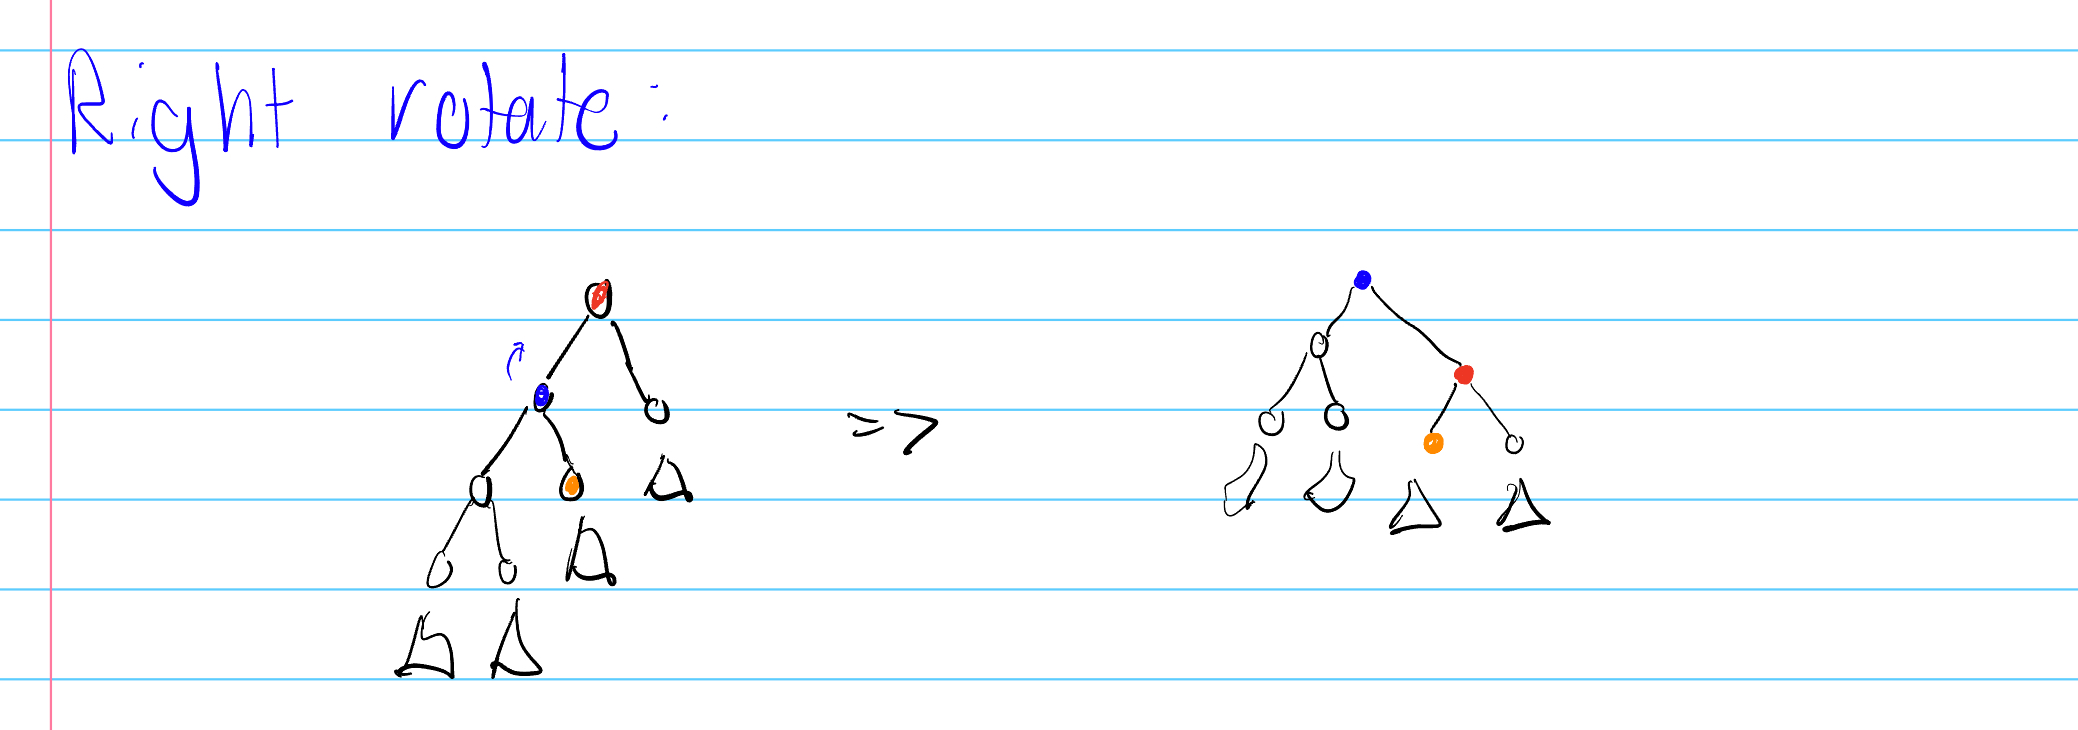
\includegraphics[scale=0.2]{graphics/Right_Rotate.jpg}
\end{figure}

In the right rotation of a node, the min/max changes for two nodes; the node we are rotating and the parent node (their ancestors will also be changed, but as we come up in our fix, we make continue to update the min/max/min-gap the same way. So either we do another rotation further up or we update the fields, in both cases we update the fields at each level). More specifically, the max value of the the node we are rotating will switch to the max value of the parent node, while the min value will remain the same. The min value of the parent node will change to the min value of the right child of the node we are rotating. The min-gap of both the parent node and the node we are rotating will be changed according to the new max and min fields of the nodes by performing the calculation for min-gap. 

\begin{figure}[htb!]
     \centering
     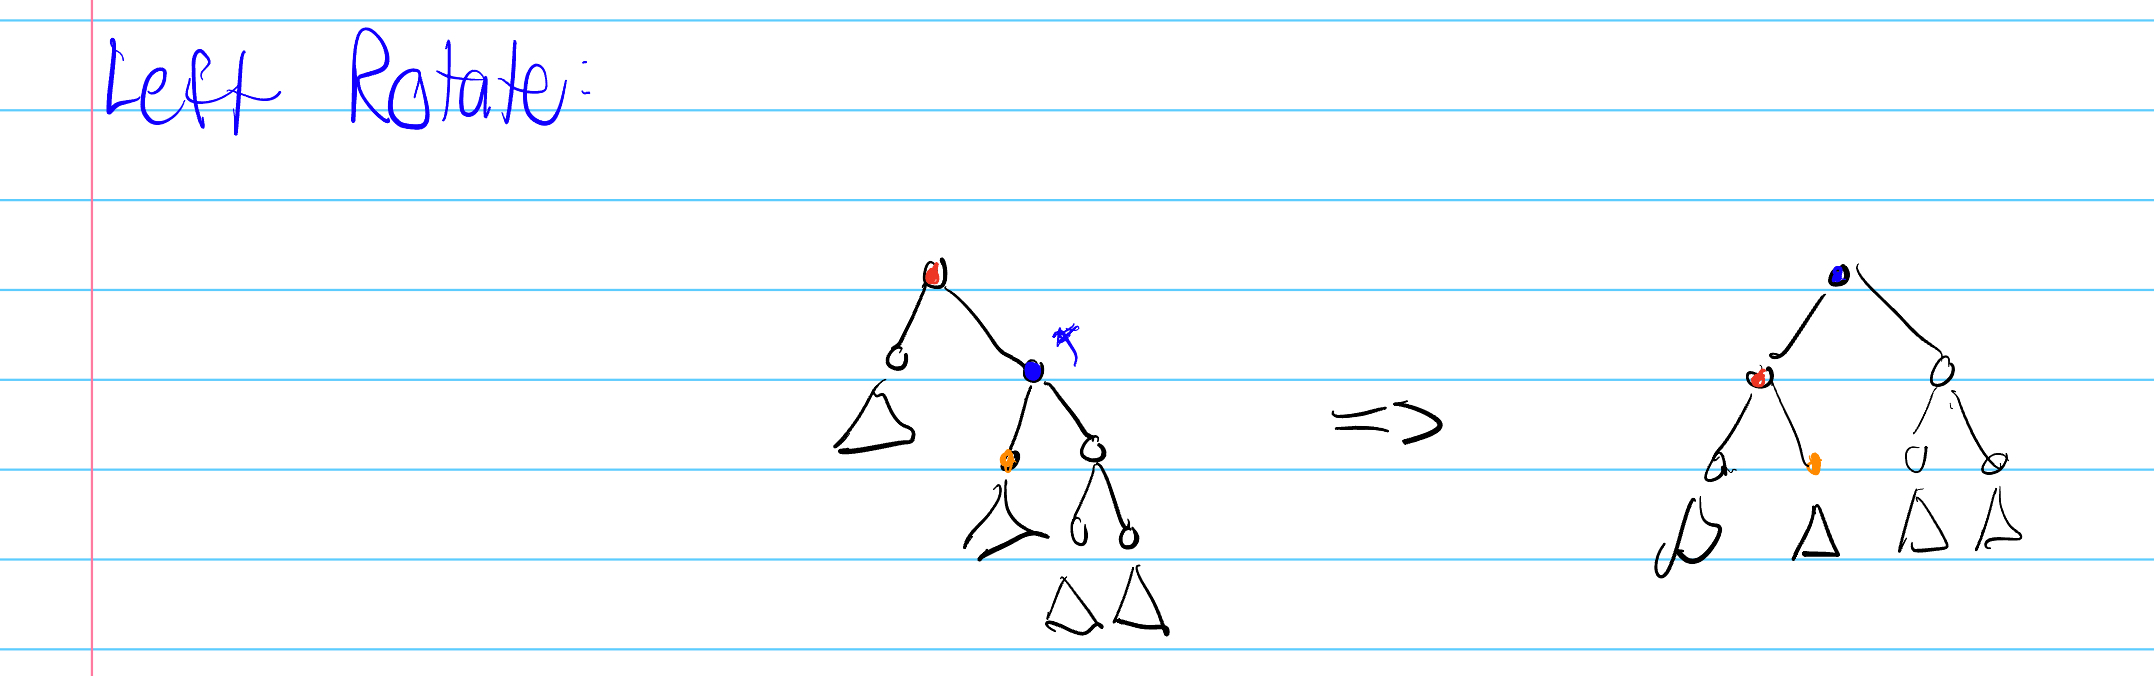
\includegraphics[scale=0.2]{graphics/Left_Rotate.jpg}
\end{figure}

The left rotation is similar to that of the right rotation. The max value of the node we are left rotating will remain the same, but its min value will change to the min value of its parent node. The min value of the parent node will remain the same, but the it's max value will change to that of the max of the left child of the node we are left rotating. Once again the min-gap changes accordingly depending on the values of the new min and max. 

Since we only change the min, max, and min-gap of 2 nodes for each rotation and there are in the worst case $O(\log n)$ rotations do be done to re-balance our red black tree which all take constant time, and updating the respective fields also takes constant time, the fix operation which runs $O(\log n )$, will also also run in $O(\log n )$. This will also hold true for the fix in deleting a node in a red black tree. 

Thus, the insertion in a dynamic set has operations that run in $O(\log n)$, so insertion takes $O(\log n)$.

\item[\sc Deletion.] The algorithm for deleting a node in a red black tree deletes a node like it would in a binary tree, and uses a fix algorithm similar to that of \textsc{Insertion}, to repair any violation of red-black tree properties that could occur. The following is an algorithm to delete a node in the BST starting from the root of the tree, 

\begin{lstlisting}[caption = deleting a node]
DELETE(rb_tree, del_node):
    y = del_node
    del_node_color = colour[y]
    if(left[del_node] == null):
        x = right[node]
        TRANSPLANT(rb_tree, node, right[node]
    else if (right[node] == null):
        x = left[node]
        TRANSPLANT(rb_tree, node, left[node])
    else:
        y = TREE-MINIMUM(right[node])
        del_node_color = y.color
        x = right[y]
        if (y != right[del_node])
            TRANSPLANT(rb_tree, y, right[y])
            right[y] = right[del_node]
            parent[right[y]] = y
        else 
            parent[x] = y

        TRANSPLANT(rb_tree, y, right[y])
        left[y] = left[del_node]
        parent[left[y]] = y 
        colour[y] = colour[del_node] 
    if (del_node_color == black):
        DELETE_FIX(rb_tree, x)
\end{lstlisting}
\begin{lstlisting}[caption = fixing a red-black tree after deletion]
DELETE_FIX(rb_tree, x):
    while x != root[rb_tree] && colour[x] == black{
        if (x == left[parent[x]]):
            y = right[parent[x]]
            if (colour[y] == red):
                colour[y] = black 
                colour[parent[x]] = red 
                ROTATE_LEFT(rb_tree, parent[x])
                y = right[parent[x]]
            if (colour[left[y]] == black && colour[right[y]] == black):
                colour[y] = red 
                x = parent[x]
            else:
                if (colour[right[y]] == black): 
                    colour[left[y]] = black 
                    colour[y] = red
                    ROTATE_RIGHT[rb_tree, y]
                    y = right[parent[x]]
                    
                colour[y] = colour[parent[x]]
                colour[parent[x]] = black 
                colour[right[y]] = black 
                ROTATE_LEFT[rb_tree, parent[x]] 
                x = root[rb_tree]
        else
            y = left[parent[x]]
            if (colour[y] == red):
                colour[y] = black 
                colour[parent[x]] = red 
                ROTATE_RIGHT(rb_tree, parent[x])
                y = right[parent[x]]
            if (colour[right[y]] == black && colour[left[y]] == black):
                colour[y] = red 
                x = parent[x]
            else:
                if (colour[left[y]] == black): 
                    colour[right[y]] = black 
                    colour[y] = red
                    ROTATE_RIGHT[rb_tree, y]
                    y = left[parent[x]]
                    
                colour[y] = colour[parent[x]]
                colour[parent[x]] = black 
                colour[left[y]] = black 
                ROTATE_RIGHT[rb_tree, parent[x]] 
                x = root[rb_tree]
    }
    colour[x] = black
    
\end{lstlisting}

\begin{figure}[htb!]
     \centering
     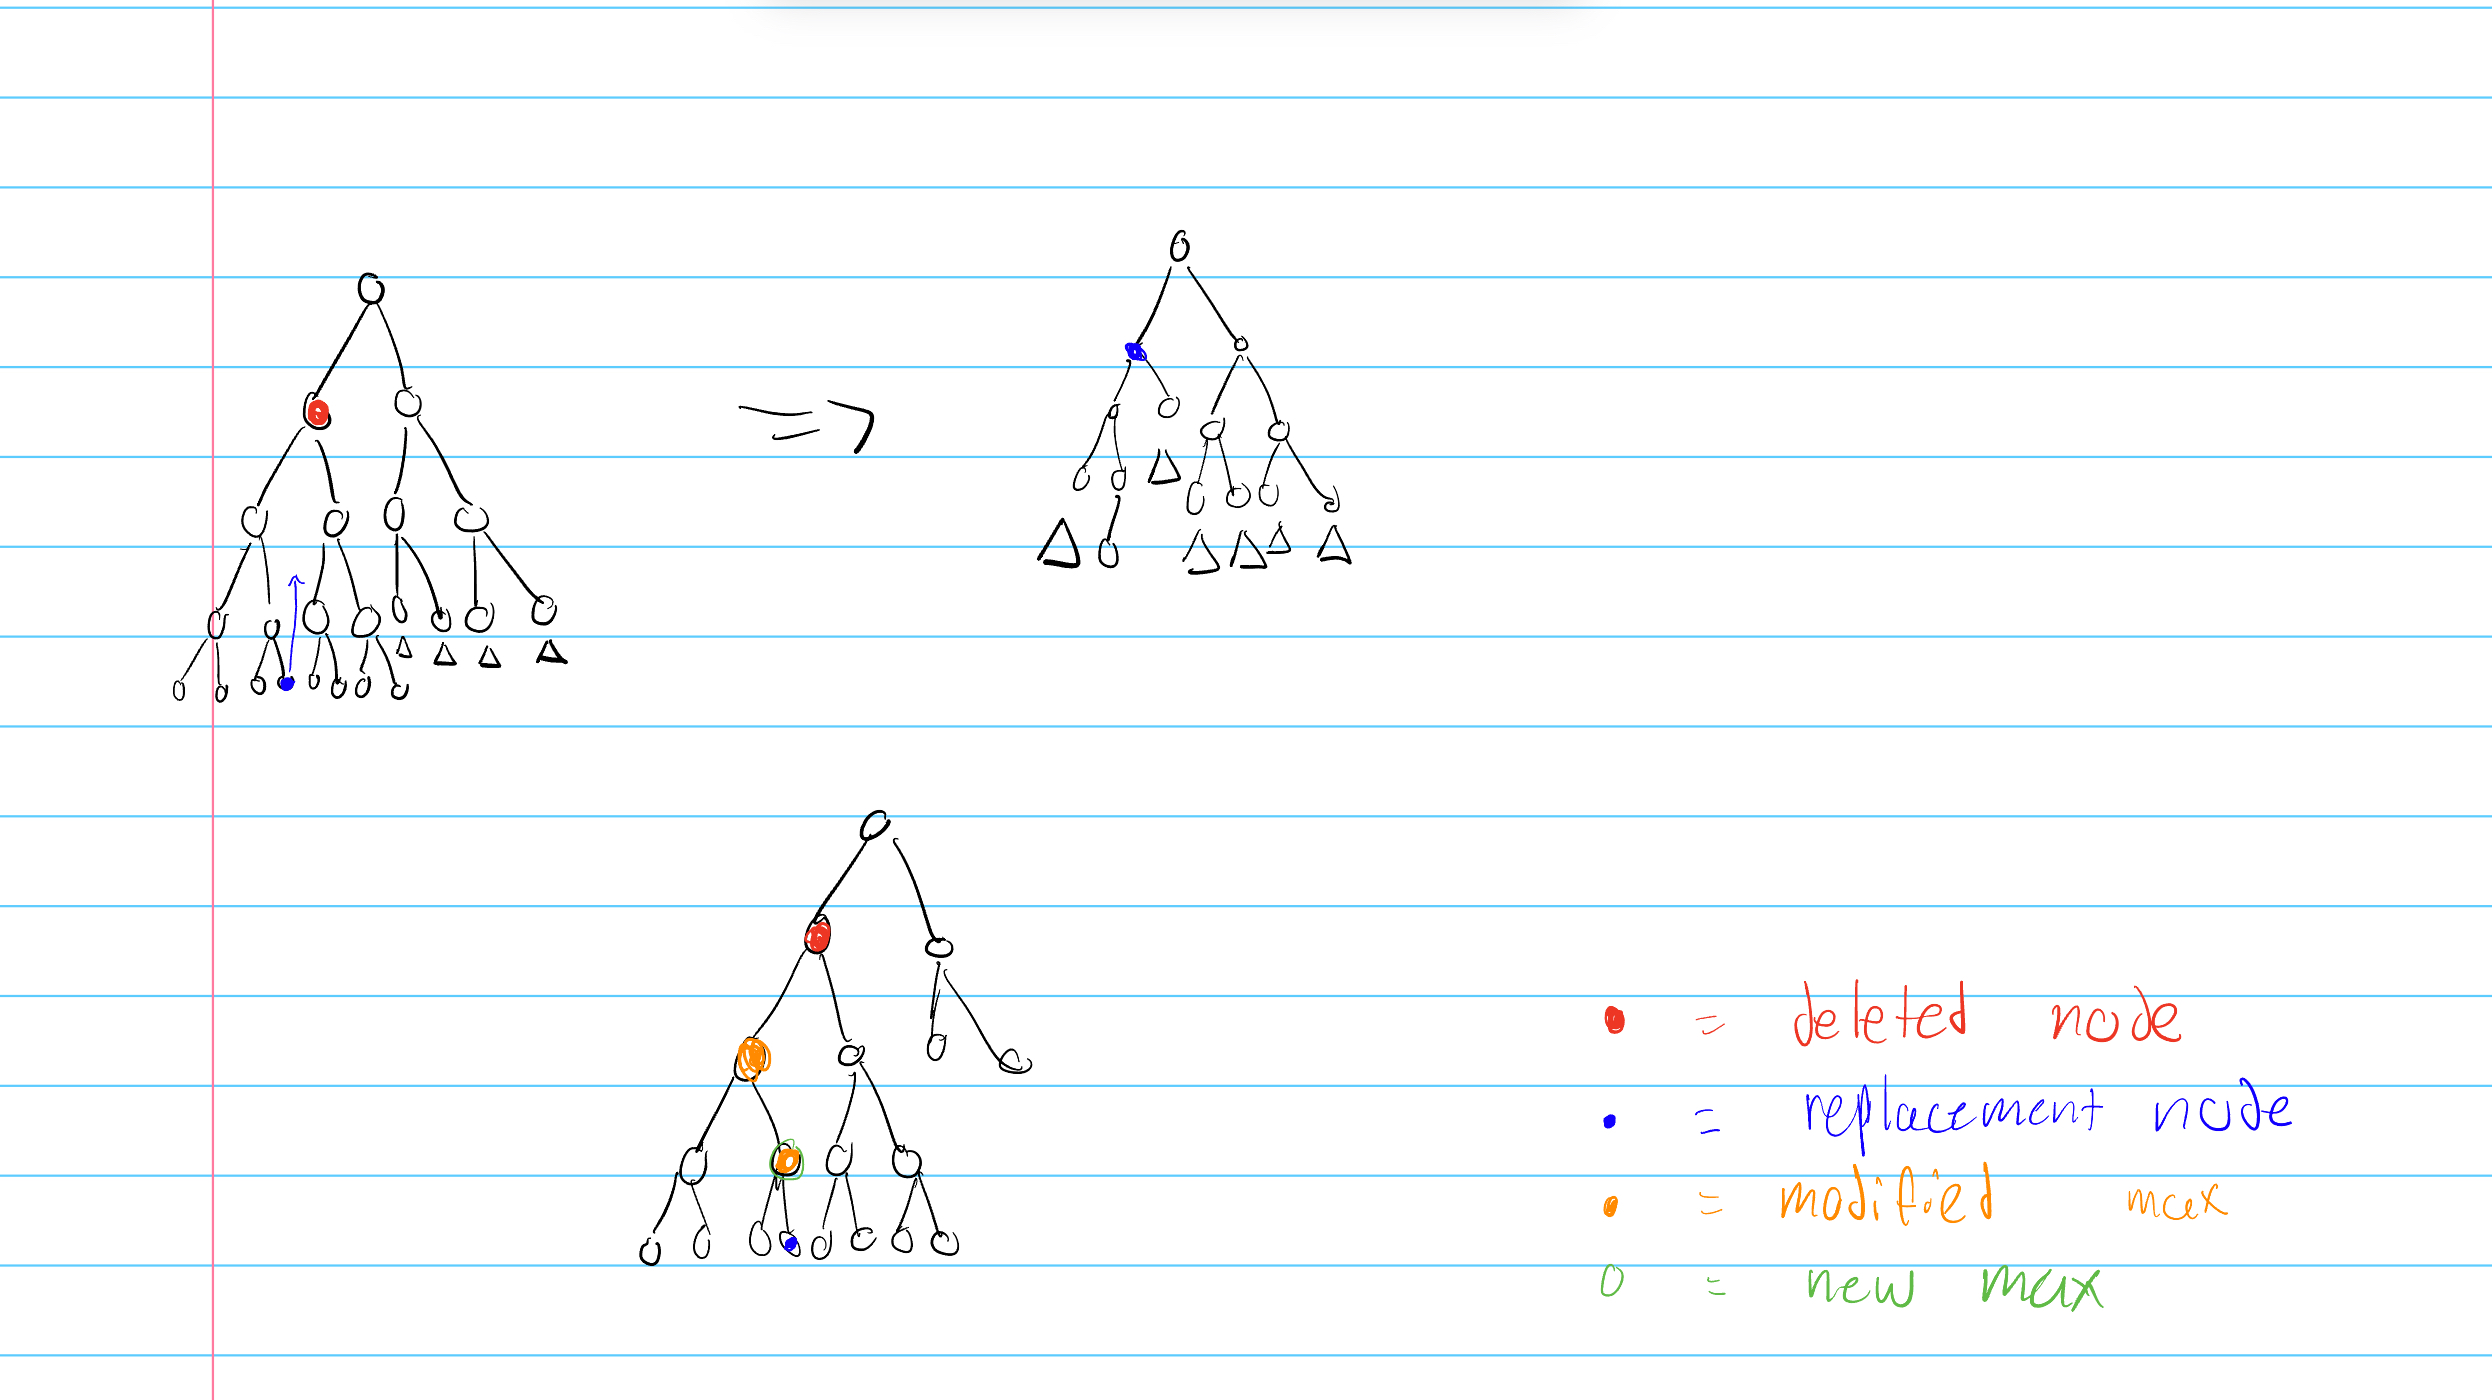
\includegraphics[scale=0.2]{graphics/Delete_diagram.jpeg}
\end{figure}

In the algorithm for deleting a node in a binary tree, we must update the min, max, and min-gap fields of each node. The delete algorithm works by first binary searching through the red black tree to find the node we delete from the red black tree, which takes at most $O(\log n)$ and replaces the deleted node with the node that has the greatest value in the left subtree (the right most node in the right subtree of the node we are deleting). The min, max, and min-gap values that will change is the node we are using to replace the deleted node, and every ancestor of our replacement node up to the node that was deleted. Each of these nodes will have a new max since their max was used to replace the deleted node. The new max of each of ancestor nodes up to the deleted node, but not including it, is the value of the parent of our replacement node(the ancestor nodes up to the root of the left subtree of the node that was deleted). The min of these nodes is not changed, so the min-gap is calculated with the new max value for every ancestor up to the root (since its children have different max/min thus potentially different min-gap). Once again, deleting a node in a red black tree takes $O(\log n)$, therefore the deleting of a node and updating of the correct fields takes $O(\log n)$ since a constant number of operations are performed at each level, so the time complexity is level dependent. Since a red black tree is balanced, it will have $O(\log n) $ levels. 

Our fix function works in a similar way as the fix for insertion, therefore the fix will take $O(\log n)$. So the entire deletion of a number in a dynamic set will take $O(\log n)$. 

The min-gap operation takes constant time since every time we change the elements in our dynamic set, we adjust the min-gap of nodes that were affected by an operation, and every ancestor that is influenced by the affected nodes, so the min-gap can be retrieved from the root node. So it takes constant time, $O(1)$ to find the min-gap of the dynamic set.
\item[\sc Search.]
Searching for a node in red black tree takes $O(\log n)$ since the tree is always balanced, so it would take $O(\log n)$ to find an element in the dynamic set. The search algorithm is the following, 

\begin{lstlisting}
    def search_redblack(rb_tree, key_tofind):
        if key[rb_tree] > key_tofind:
            search_redblack(left[rb_tree], key_tofind)
        if key[rb_tree] < key_tofind:
            search_redblack(right[rb_tree], key_tofind)
        else:
            return rb_tree, key[rb_tree]
\end{lstlisting}
\item[\sc Min-gap.] Lastly, considering all of the previously mentioned points, it follows that since the min-gap of our set of numbers is a "field" of the tree, accessing it requires constant time. In order to maintain its accuracy, it is updated whenever the tree is altered. 
\end{enumerate}
\newpage 
\item \textsc{The node of smallest tension in a tree.} Given is an unrooted free tree of size $n$.
The nodes are labeled from $1$ to $n$, and for each node, we have a linked list of its neighbors. When a node $u$ is deleted, it breaks the tree up into a forest of disjoint trees, say $T_1, ... , T_k$. Let the sizes of these trees be denoted by $|T_1|,... , |T_k|$. We define the tension of $u$ as $\max_{1 \leq i \leq k} T_i$. The objective is to find a node $u$ of smallest tension. Intuitively, it should be near the “center” of the tree. Write an algorithm
that takes $O(n)$ worst-case time.
\sol 
See the algorithm on the next page. The complexity is easily seen to be $O(n)$, given that line 21 executes at most $n$ times, and both loops at lines 28 and 34 iterate $n$ times. Additionally, the post\_order\_traversal function is $O(n)$, as it traverses every node in the tree. 

The algorithm uses the following data structure, 
\begin{equation*}
  \begin{split}
    &\texttt{struct NODE}\\ 
    &\{\\ 
    &\texttt{linkedList } \text{neighbour}; \\ 
    &\texttt{int } \text{tension}; \\ 
    &\texttt{int } \text{size} ;\\ 
    &\texttt{bool }\text{visited}; \\
    &\}\\
  \end{split}
\end{equation*}

\begin{algorithm}
    \caption{Smallest Tension}
    \SetKwProg{Fn}{Function }{\string:}{}
    \SetKwInput{KwOut}{Output}
    \SetKwInput{KwIn}{Input}
    \SetKwFunction{stru}{struct}
    \SetKwData{true}{True}
    \SetKwData{chi}{child}
    \SetKwData{parent}{parent}
    \SetKwData{ten}{tension}
    \SetKwData{size}{size}
    \SetKwData{visited}{visited}    
    \SetKwData{root}{root}
    \SetKwData{toproot}{TopRoot}
    \SetKwData{nei}{neighbours}   
    \SetKwData{false}{False}  
    \SetKwData{null}{NULL}   
    \SetKwFunction{mn}{MAKENULL}
    \SetKwFunction{top}{PEEK}
    \SetKwFunction{pop}{POP}
    \SetKwFunction{isemp}{ISEMPTY}
    \SetKwFunction{potrav}{post\_order\_traversal}
    \SetKwFunction{exit}{exit}
    \SetKwFunction{init}{initialize}
    \SetKwData{temp}{temp}
    \SetKwData{continue}{continue}

    \KwIn{A list $\Omega := \{1,2,3,...,n\}$ of nodes, and for each node, a linked list of neighbours.}
    \KwOut{The node of minimum tension.}
\BlankLine
\Fn{\potrav{\root}}{
    $\root.\visited \gets \true;$\\
    \If{$|\root.\nei| = 1$}{
        $\root.\size \gets 1; $\\ 
        $\root.\ten \gets n-1;$\\
        \Return ;
    }
    \ForAll{ \texttt{NODE} $\chi$ in $\root.\nei$}{
        \If{$\chi.\visited = \true$}{\continue\tcp{\color{blue} means the node is a parent, so don't visit.}}
        \potrav{$\chi$};
    }
    \tcp{\color{blue}visit node}
    
    \ForAll{ \texttt{NODE} $\chi$ in $\root.\nei$}{
        $\root.\size \gets \root.\size + \chi.\size$; \tcp{\color{blue}one of the nodes is going to be the parent, but since it hasn't been visited yet, its field \texttt{size} will be 0, so this is an accurate calculation of the size.}
    }
    $\root.\ten \gets \max \{\max_{i \in \root.\nei} \{i.\size\}, n - \root.\size\} $;\\ 
    \Return; 
  } \tcp{\color{red}--- Driver code ---}
 \tcp{\color{blue} add fields to each node.}
       \ForAll{$i \in \Omega$}{      
       $\temp \gets i.\nei;$\\ 
      $i \gets new \texttt{ struct } \texttt{NODE}$;\\  
      $i.\visited \gets \false;$\\ 
      $i.\nei \gets \temp ;$\\ 
      $i.\ten \gets 0;$\\ 
      $i.\size \gets 0;$
     }
    \tcp{\color{blue} find a node that's not a leaf and initialize it as root.}
    \ForAll{$i \in \Omega $}{
      \If{$|i.\nei| >1$}{
      $\toproot \gets i;$\\ 
      \exit;
      }
    }
    \tcp{\color{blue} call the traversal at the top root}
    $\potrav(\toproot)$;\\
    $\temp \gets \infty ;$\\ 
    \tcp{\color{blue}find the node of minimum tension}
    \For{all $i\in \Omega$}{
      \If{$i.\ten < \temp$}{
        $\temp \gets i.\ten$;
      }
    }
    \Return $\temp;$
    \end{algorithm}

\end{enumerate}
\end{document}
